\section{Simulation Analysis}
\label{sec:simulation}

\indent

This section discusses the circuit simulation, performed using {\it Ngspice}. 

This circuit was entered into the {\it Ngspice} simulation environment. This tool is used to simulate analog electronic circuits and predict circuit behaviour. 
This {\it Ngspice} simulation begins by defining the ground node, which is the node with potential 0 (by convention). In {\it Ngspice}, the ground node is represented by $V_0$. In our theoretical analysis, the ground node was defined to be node 4. However node 4 is still needed because we must introduce a voltage source with 0V potential, in order to measure the current Ic for the dependent voltage source, since {\it Ngspice} considers the voltage sources as Ammeters.
The new diagram, which represents more accurately what was introduced in {\it Ngspice}, is shown on Figure~\ref{fig:ngspiceCircuit}.

\begin{figure}[h] \centering
    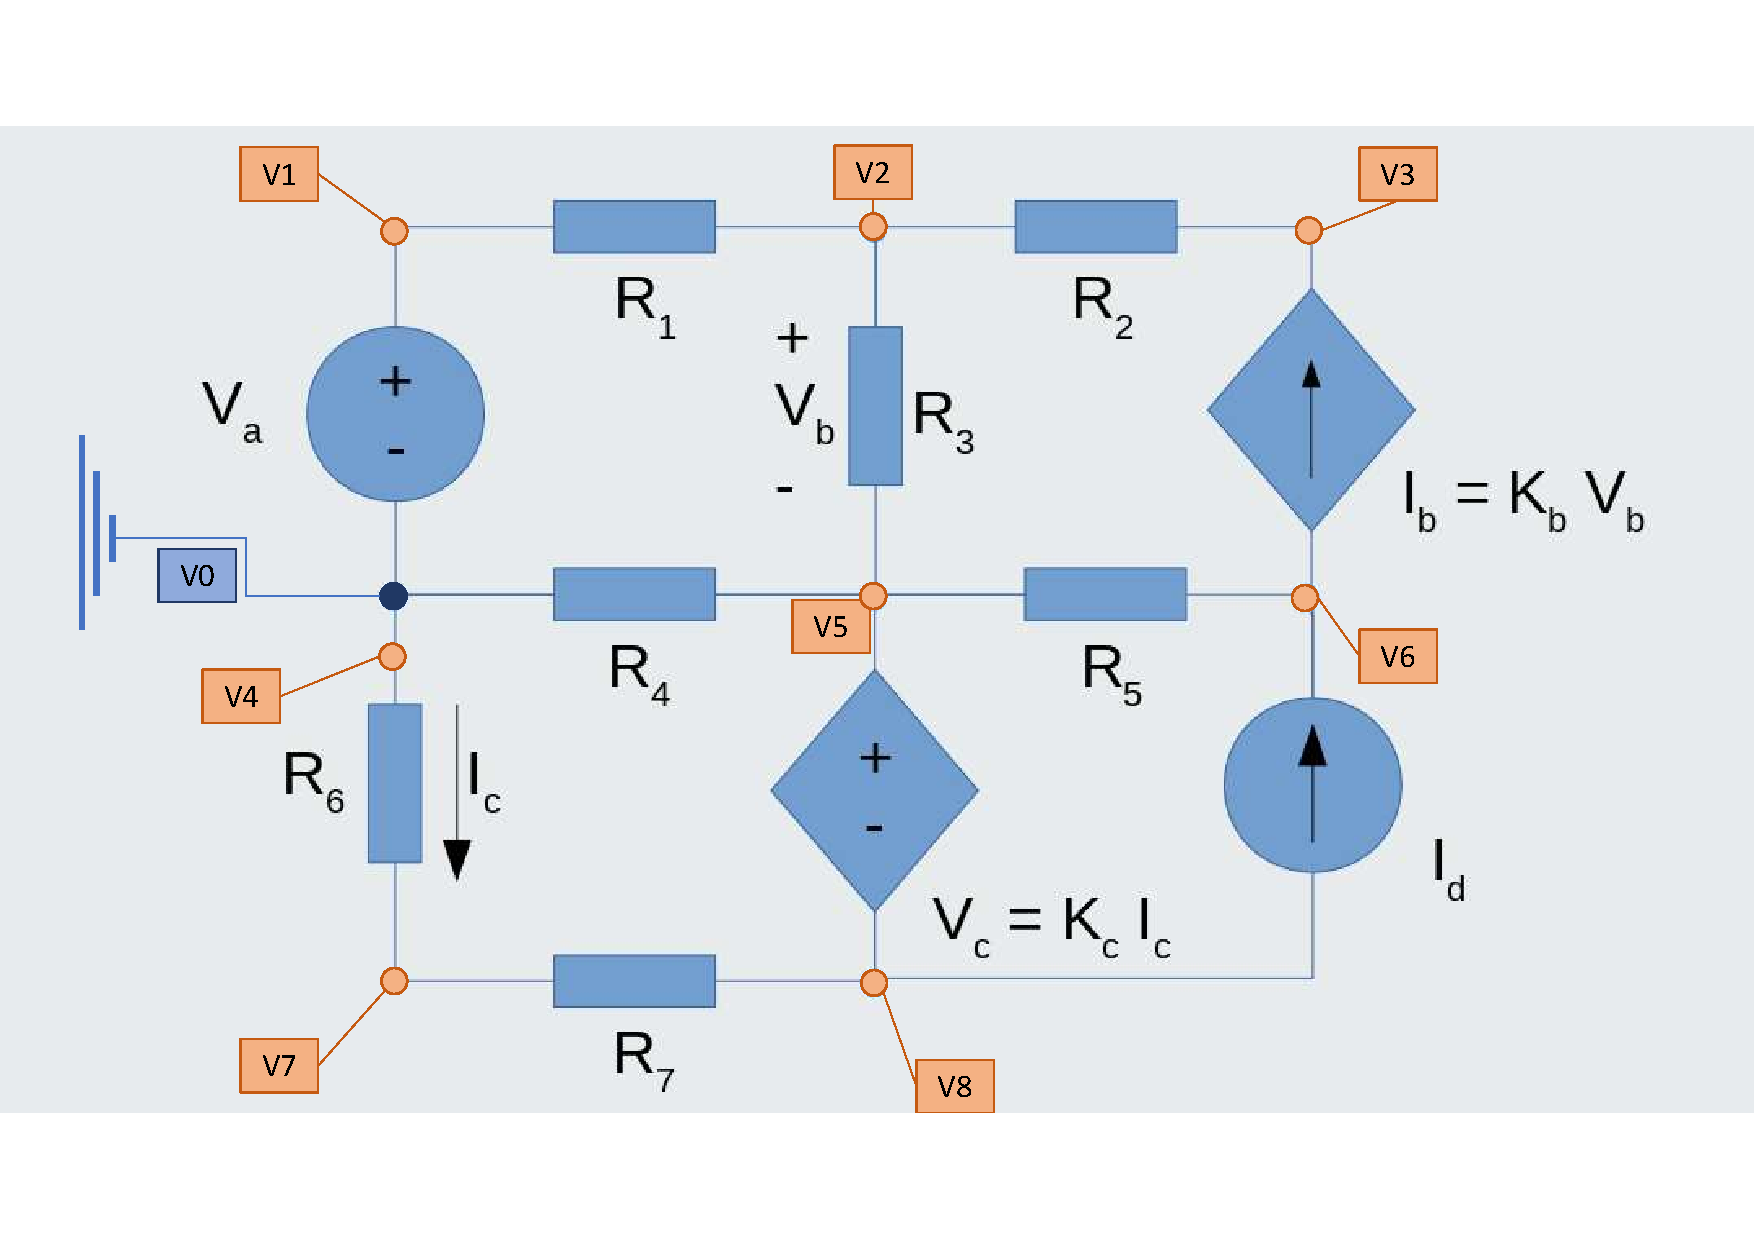
\includegraphics[width=0.8\linewidth]{Images/ngspice model.pdf}
    \caption{Voltage and Current driven circuit with 7 resistors.}
    \label{fig:ngspiceCircuit}
\end{figure}





Table~\ref{tab:op} shows the simulated operating point results for the circuit
under analysis.

\begin{table}[h]
  \centering
  \begin{tabular}{|l|r|}
    \hline    
    {\bf Name} & {\bf Value [A or V]} \\ \hline
    @c[i] & 0.000000e+00\\ \hline
@gcs[i] & -2.04136e-04\\ \hline
@r1[i] & 1.945229e-04\\ \hline
@r2[i] & -2.04136e-04\\ \hline
@r3[i] & -9.61363e-06\\ \hline
@r4[i] & 1.156284e-03\\ \hline
@r5[i] & 2.041365e-04\\ \hline
@r6[i] & 9.617613e-04\\ \hline
@r7[i] & 9.617613e-04\\ \hline
v(1) & 5.008942e+00\\ \hline
v(2) & 4.808960e+00\\ \hline
v(3) & 4.394159e+00\\ \hline
v(4) & 0.000000e+00\\ \hline
v(5) & 4.837862e+00\\ \hline
v(6) & 5.474755e+00\\ \hline
v(7) & -2.00872e+00\\ \hline
v(8) & -2.97092e+00\\ \hline

  \end{tabular}
  \caption{Operating point. A variable preceded by @ is of type {\em current}
    and expressed in Ampere; other variables are of type {\it voltage} and expressed in
    Volt.}
  \label{tab:op}
\end{table}







